\documentclass[12pt, letterpaper] {article}

\parindent=5mm
\usepackage[spanish]{babel}

\usepackage{amssymb}
\usepackage{amsmath} 
\usepackage{amsfonts}

\usepackage[numbers,sort&compress]{natbib}
\usepackage{graphicx}

\usepackage{url}
\usepackage{hyperref}

\usepackage[top=25mm, bottom=20mm, left=1.5cm, right=1.5cm]{geometry}
\setlength{\parskip}{2mm}
\setlength{\parindent}{1pt}

\usepackage{listings}

\usepackage{float}

\usepackage[utf8]{inputenc}
\usepackage{graphicx} 
\usepackage{subfigure} 

\usepackage{color}
\usepackage{multirow}

\definecolor{dkgreen}{rgb}{0,0.6,0}
\definecolor{gray}{rgb}{0.5,0.5,0.5}
\definecolor{mauve}{rgb}{0.58,0,0.82}

\usepackage{color}
\usepackage{listings}
\lstset{ %
  language=R,                     % the language of the code
  basicstyle=\footnotesize,       % the size of the fonts that are used for the code
  numbers=left,                   % where to put the line-numbers
  numberstyle=\tiny\color{gray},  % the style that is used for the line-numbers
  stepnumber=1,                   % the step between two line-numbers. If it's 1, each line
                                  % will be numbered
  numbersep=5pt,                  % how far the line-numbers are from the code
  backgroundcolor=\color{white},  % choose the background color. You must add \usepackage{color}
  showspaces=false,               % show spaces adding particular underscores
  showstringspaces=false,         % underline spaces within strings
  showtabs=false,                 % show tabs within strings adding particular underscores
  frame=single,                   % adds a frame around the code
  rulecolor=\color{black},        % if not set, the frame-color may be changed on line-breaks within not-black text (e.g. commens (green here))
  tabsize=2,                      % sets default tabsize to 2 spaces
  captionpos=b,                   % sets the caption-position to bottom
  breaklines=true,                % sets automatic line breaking
  breakatwhitespace=false,        % sets if automatic breaks should only happen at whitespace
  title=\lstname,                 % show the filename of files included with \lstinputlisting;
                                  % also try caption instead of title
  keywordstyle=\color{blue},      % keyword style
  commentstyle=\color{dkgreen},   % comment style
  stringstyle=\color{mauve},      % string literal style
  escapeinside={\%*}{*)},         % if you want to add a comment within your code
  morekeywords={*,...}            % if you want to add more keywords to the set
} 

\usepackage{booktabs}
\usepackage[table,xcdraw]{xcolor}


\author{Ricardo Rosas Macías}

\title{Práctica 1. Movimiento Browniano}

\date{\today}

\begin{document}

\maketitle


\begin{abstract}
Con fines educativos se hizó la práctica con el fin de observar la trayectoria que puede tener el movimiento de una nanopartícula o mejor conocido como movimiento Browniano. El software R permitió emular el movimiento de manera aleatoria, asimismo realizar la medición de manera cuantitativa, de su distancia Euclidiana y Manhattan.\\[5mm]
\end{abstract}

\section{Introducción}

El movimiento Browniano es el desplazamiento aleatorio que una partícula o nanopartícula efectúa en un medio. En el experimento que se llevó acabo, la distancia que recorre la nanopartícula se encuentra cuantificada en discretos, de tal forma que cada paso tenga el mismo tamaño. La ejecución del código tiene el interés práctico de conocer la posición de la partícula respecto al origen. 

 \section{Objetivo}
La finalidad de la simulación del movimiento Browniano es discernir si la nanopartícula regresa al origen, además con el procesamiento de datos permitirá determinar si los parámetros afectan en el comportamiento.
 
  \subsection{Descripción}

Lo que se debe hacer es \cite{elisawebMB}:
\begin{quotation}
 ``Examinar de manera sistemática los efectos de la dimensión en la probabilidad de regreso al origen del movimiento Browniano para dimensiones 1 a 8 en incrementos lineales de uno, variando el número de pasos de la caminata como potencias de dos con exponente de 6 a 12 en incrementos lineales de uno, con 30 repeticiones del experimento para cada combinación.\\
 
 El primer reto es estudiar de forma sistemática y automatizada el tiempo de ejecución de una caminata (en milisegundos) en términos del largo de la caminata (en pasos) y la dimensión.\\

El segundo reto es realizar una comparación entre una implementación paralela y otra versión que no aproveche paralelismo en términos del tiempo de ejecución, aplicando una prueba estadística adecuada para determinar si la diferencia es significativa.''
\end{quotation}

\section{Resultados y conclusiones}

Para obtener los resultados se le realizaron modificaciones al código anteriormente reportado \cite{AsP1}\cite{MPP1}, como se muestra en la parte inferior. En las primeras líneas se indica los incrementos de pasos de $2^6$ a $2^{12}$; que esta representada por la variable pasos, así como  las 30 repeticiones que efectuara. Además el código esta paralelizado de modo que permita una ejecución más rápida, en las dimensiones 1 a 8. 


\begin{lstlisting}[language=R]
rep <- 30
pasos <- sapply(6:12, function(x) {2**x})
eucl <- FALSE

cluster <- makeCluster(detectCores() - 1)
clusterExport(cluster, "dur")
clusterExport(cluster, "eucl")
clusterExport(cluster, "pasos")
datos <- data.frame()
for (dur in pasos) {
  for (dimension in 1:8) {
    counter <- 0
    clusterExport(cluster, "dimension")
    resultado <- parSapply(cluster, 1:rep,
                           function(r) {
                             pos <- rep(0, dimension)
                             test <- rep(0, dimension)
                             mayor <- 0
                             counter <- 0
                             for (t in 1:dur) {
                               cambiar <- sample(1:dimension, 1)
                               cambio <- 1
                               if (runif(1) < 0.5) {
                                 cambio <- -1
                               }
                               pos[cambiar] <- pos[cambiar] + cambio
                               if (eucl) {
                                 d <- sum(sqrt(pos**2))
                               } else { # Manhattan
                                 d <- sum(abs(pos))
                               }
                               if (d > mayor) {
                                 mayor <- d
                               }
                               if (all(pos==test)){
                                 counter <- counter + 1
                               } 
                             }
                             return(counter)
                           })
    datos <- rbind(datos, resultado)
  }
}
stopCluster(cluster)
Adata <- data.frame(datos) 
\end{lstlisting}

Con ayuda de la paquetería \textit{ggplot2} \cite{Bxplot}\cite{BPlot}, se obtuvo la visualización de código anterior. En la figura \ref{PS} muestra que conforme avanzan las dimensiones los datos tienen más dispersión central, por lo que hay algunos datos atípicos que aparecen en forma de puntos en los gráficos que están fuera del rango intercuartílico. Por lo tanto hay más probabilidad de que los dos parámetros afectan al comportamiento de la nanopartícula.


\begin{figure}[H]
\centering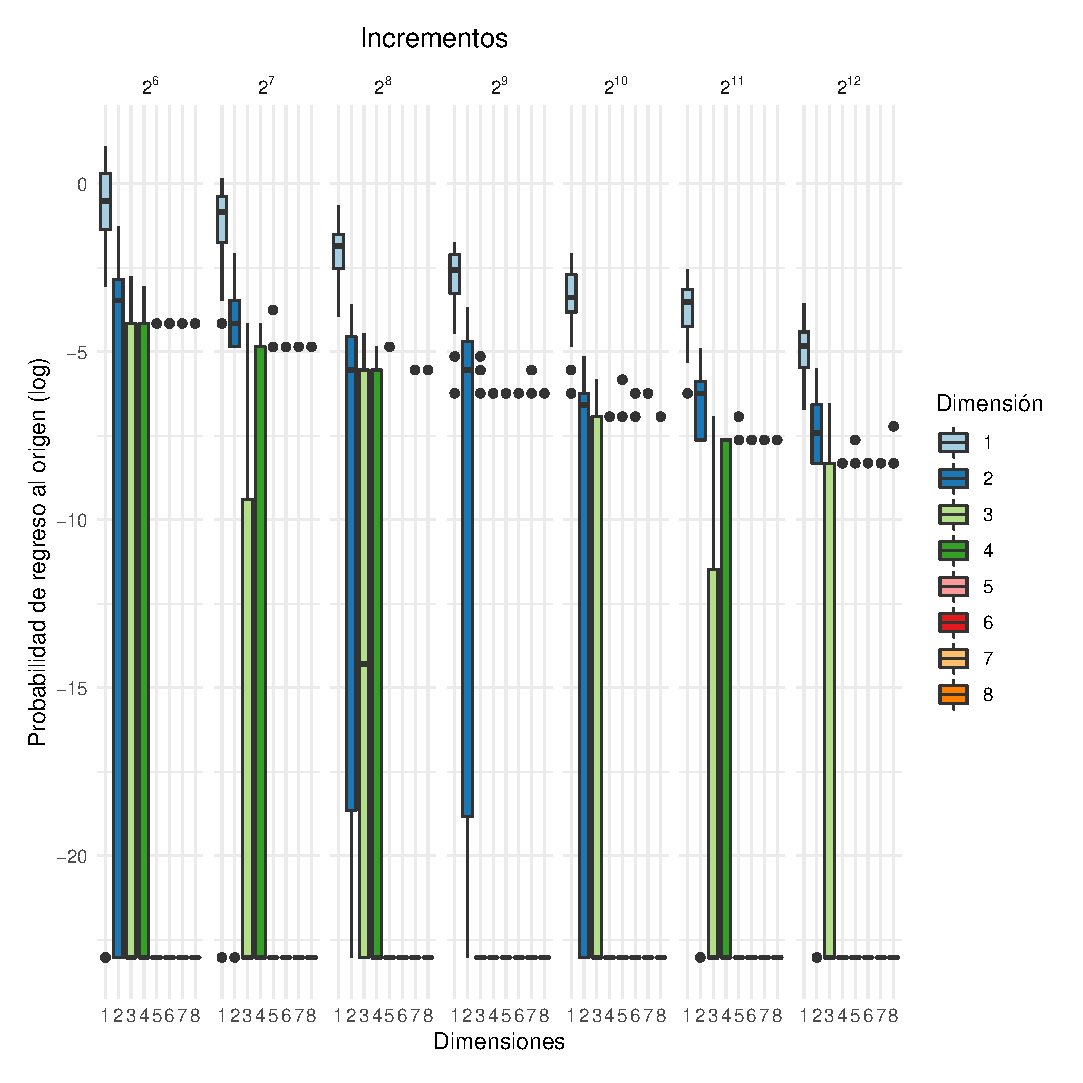
\includegraphics[width=111mm]{d_Manh.eps}
\caption{Distancia Manhattan de partícula en incrementos de $2^6$ a $2^{12}$}
\label{PS}
\end{figure}

\subsection{Reto 1}

Para el primer reto se creo un código respecto a la literatura \cite{P1JA}, con la intención de conocer el tiempo de ejecución respecto a la caminata que la nanopartícula realiza en 100 pasos.

\begin{lstlisting}[language=R]
rep <- 1
dur <- 100
dim <- 8
orig <- rep(0, dim)
tab <- numeric(length(rep*dim))
elapsed <- numeric(length(dur))
i = 1
j = 1
anterior <- 0
timeT <- system.time(
  for (dimension in dim:dim) {
    timeDim <- system.time(
      for (repeticion in 1:rep)  { 
        cero <- 0              
        pos <- rep(0, dimension)
        for (t in 1:dur) {
          timeD <- system.time(
           for (x in 1:1) {
            cambiar <- sample(1:dimension, 1)                     
             if (runif(1) < 0.5) {
                cambio <- 1
              } else {
                cambio <- -1
              }
              pos[cambiar] <- pos[cambiar] + cambio
              if (all (pos == orig)) {
                cero = cero + 1
              }
           })[3]
        time <- (timeD + anterior)
         elapsed[j] <- time
         anterior <- time
          j = j + 1
        }
        prob <- ((cero/dur)*100)
        tab[i] <- prob
        i = i + 1
      })[3]
  })
  \end{lstlisting}


En la figura \ref{PSol} se puede apreciar el comportamiento creciente del tiempo respecto a incremento en los pasos, esto nos indica que al tener una caminata más grande el tiempo tendrá una tendencia a aumentar. 

\begin{figure}[H]
\centering\includegraphics[width=82mm]{tiempo.png}
\caption{Porcentaje de soluciones}
\label{PSol}
\end{figure}


\subsection{Reto 2}

Por último se realizó el reto 2 con el fin de diferenciar el cambio de tiempo de ejecución al paralelizar el código. 

\begin{lstlisting}[language=R]
library(parallel)

PSprocess <- Sys.time()
repetir <- 30 
dur <-200 
dimen <- 1:8

cluster <- makeCluster(detectCores() - 1)
clusterExport(cluster, "dur")
datos <-  data.frame()

for (dim in dimen) {
  clusterExport(cluster, "dim")
  resultado <- parSapply(cluster, 1:repetir,
                         function(x) {
                           pos <- rep(0, dim)
                           origen <- rep(0, dim)
                           contador <- 0
                           for (t in 1:dur) {
                             cambiar <- sample(1:dim, 1)
                             cambio <- 1
                             if (runif(1) < 0.5) {
                               cambio <- -1
                             }
                             pos[cambiar] <- pos[cambiar] + cambio
                             d <- dist(pos)
                             if (sum(pos == origen) == dim) {
                               contador <-  contador + 1
                             }
                           }
                           return(contador)
                         }
  )
  datos <- rbind(datos, resultado)
}
stopCluster(cluster)

PEprocess <- Sys.time()
TimeP <- PEprocess - PSprocess
print(TimeP)

Sprocess <- Sys.time()
datos <-  data.frame()
for (dim in dimen) {
  resultado <- sapply(1:repetir,
                      function(x) {
                        pos <- rep(0, dim)
                        origen <- rep(0, dim)
                        contador <- 0
                        for (t in 1:dur) {
                          cambiar <- sample(1:dim, 1)
                          cambio <- 1
                          if (runif(1) < 0.5) {
                            cambio <- -1
                          }
                          pos[cambiar] <- pos[cambiar] + cambio
                          d <- dist(pos)
                          if (sum(pos == origen) == dim) {
                            contador <-  contador + 1
                          }
                        }
                        return(contador)
                      }
  )
  datos <- rbind(datos, resultado)
}

Eprocess <- Sys.time()
TimeSP <- Eprocess - Sprocess
print(TimeSP)

vstime <- data.frame(TimeSP, TimeP)
print(vstime)
ftc <- kruskal.test(vstime)
ftc$p.value
ftc$p.value < 0.05
\end{lstlisting}

En el cuadro \ref{dattabla} se encuentran los resultados del código anterior, donde se observa una diferencia de  0.0584 segundos menos al paralelizar. Asimismo se obtuvieron resultados de la prueba estadística \textit{Shapiro-Wilk test} del código anterior, en dónde se puede notar una diferencia en el valor $p< 0.05$. Por lo tanto se puede concluir que la diferencia es minima. 

\begin{table}[H]
\caption{Comparación de tiempo de ejecución, normal versus paralelizada.}
\label{dattabla}
\centering\begin{tabular}{@{}lllll@{}}
\toprule
\cellcolor[HTML]{ECF4FF}TimeSP (Seg) & \cellcolor[HTML]{ECF4FF}TimeP (Seg) & \cellcolor[HTML]{ECF4FF}ftc\$p.value & \cellcolor[HTML]{ECF4FF}ftc\$p.value \textless 0.05 &  \\ \midrule
\cellcolor[HTML]{EFEFEF}2.020045     & \cellcolor[HTML]{EFEFEF}1.961556    & \cellcolor[HTML]{EFEFEF}0.3173105    & \cellcolor[HTML]{EFEFEF}FALSE                       &   \\ \bottomrule
\end{tabular}
\end{table}


\bibliographystyle{plainnat}

\bibliography{BHWP1}


\end{document} 